\section{Translating Wasm-DSL into AL}\label{sec:translate}

In this section, we describe the translation process of Wasm-DSL into AL.

Wasm-DSL can express whole standard of the WebAssembly, including not only
execution semantics but also syntax and validation rules.
Since generating prose from execution semantics is the main goal of this paper,
we will only focus on how execution semantics of Wasm is expressed using Wasm-DSL, but not syntax or validation.

Two kinds of \textit{definitions} are needed to express the execution semantics of Wasm:
reduction rules and auxiliary helper functions.

\subsection{Notations}
Here, we formally define the notations for the reduction rules and the auxiliary helper functions.

A reduction rule $\ruleW \in \rulesW = \configsW \times \configsW \times \premsW^\ast$ is a triplet of a
configuration \textit{lhs}, a configuration \textit{rhs}, and a finite sequences of premises \textit{prem}*.

A configuration $\configW \in \configsW = E_\bot \times E$ is a tuple of an optional expression for state \textit{s},
and an expression for a finite sequence of Wasm instructions, \textit{winstrs}.

A premise $p \in \premsW = B \uplus \{otherwise\}$ is either a boolean expression, or a
single `otherwise` whose high-level interpretation is "negation of all previous premises".

\textbf{Example.} Recall the semantics of `ref.is\_null` in figure~\ref{fig:dsl1}.
The first rule will be parsed into the following reduction rule:
\[r_1=(\bot, [val, \text{REF.IS\_NULL}]), (\bot, [\text{CONST I32 1}]), [val = (\text{REF.NULL rt})]\]
The second rule will be parsed into the following:
\[r_2=(\bot, [val, \text{REF.IS\_NULL}]), (\bot, [\text{CONST I32 0}]), [otherwise]\]
Note that both of lhs and rhs for both rules are omitting the state expression,
and thus we notate it by using $\bot$.

The high-level interpretation of a reduction rule $r = (lhs, rhs, prem*)$ should be straightforward:
when the current configuration of the program mathces \textit{lhs} and all \textit{prem}s are
evaluated to be true, then alter the program configuration into \textit{rhs}.

A helper function $\helperW \in \helpersW = NAME \times E^\ast \times E \times \premsW^\ast$ is a quadraple of
the name, parameters \textit{params}, a return expressions \textit{ret}, and a finite sequences of premises \textit{prem}*.

\textbf{Example.} \inred{TODO: Give a example of a helper function}

\subsection{Transformation}
In this section, we describe the transformation of \dsl~into \al.

\begin{figure}
  \centering
  \begin{subfigure}[b]{0.9\textwidth}
    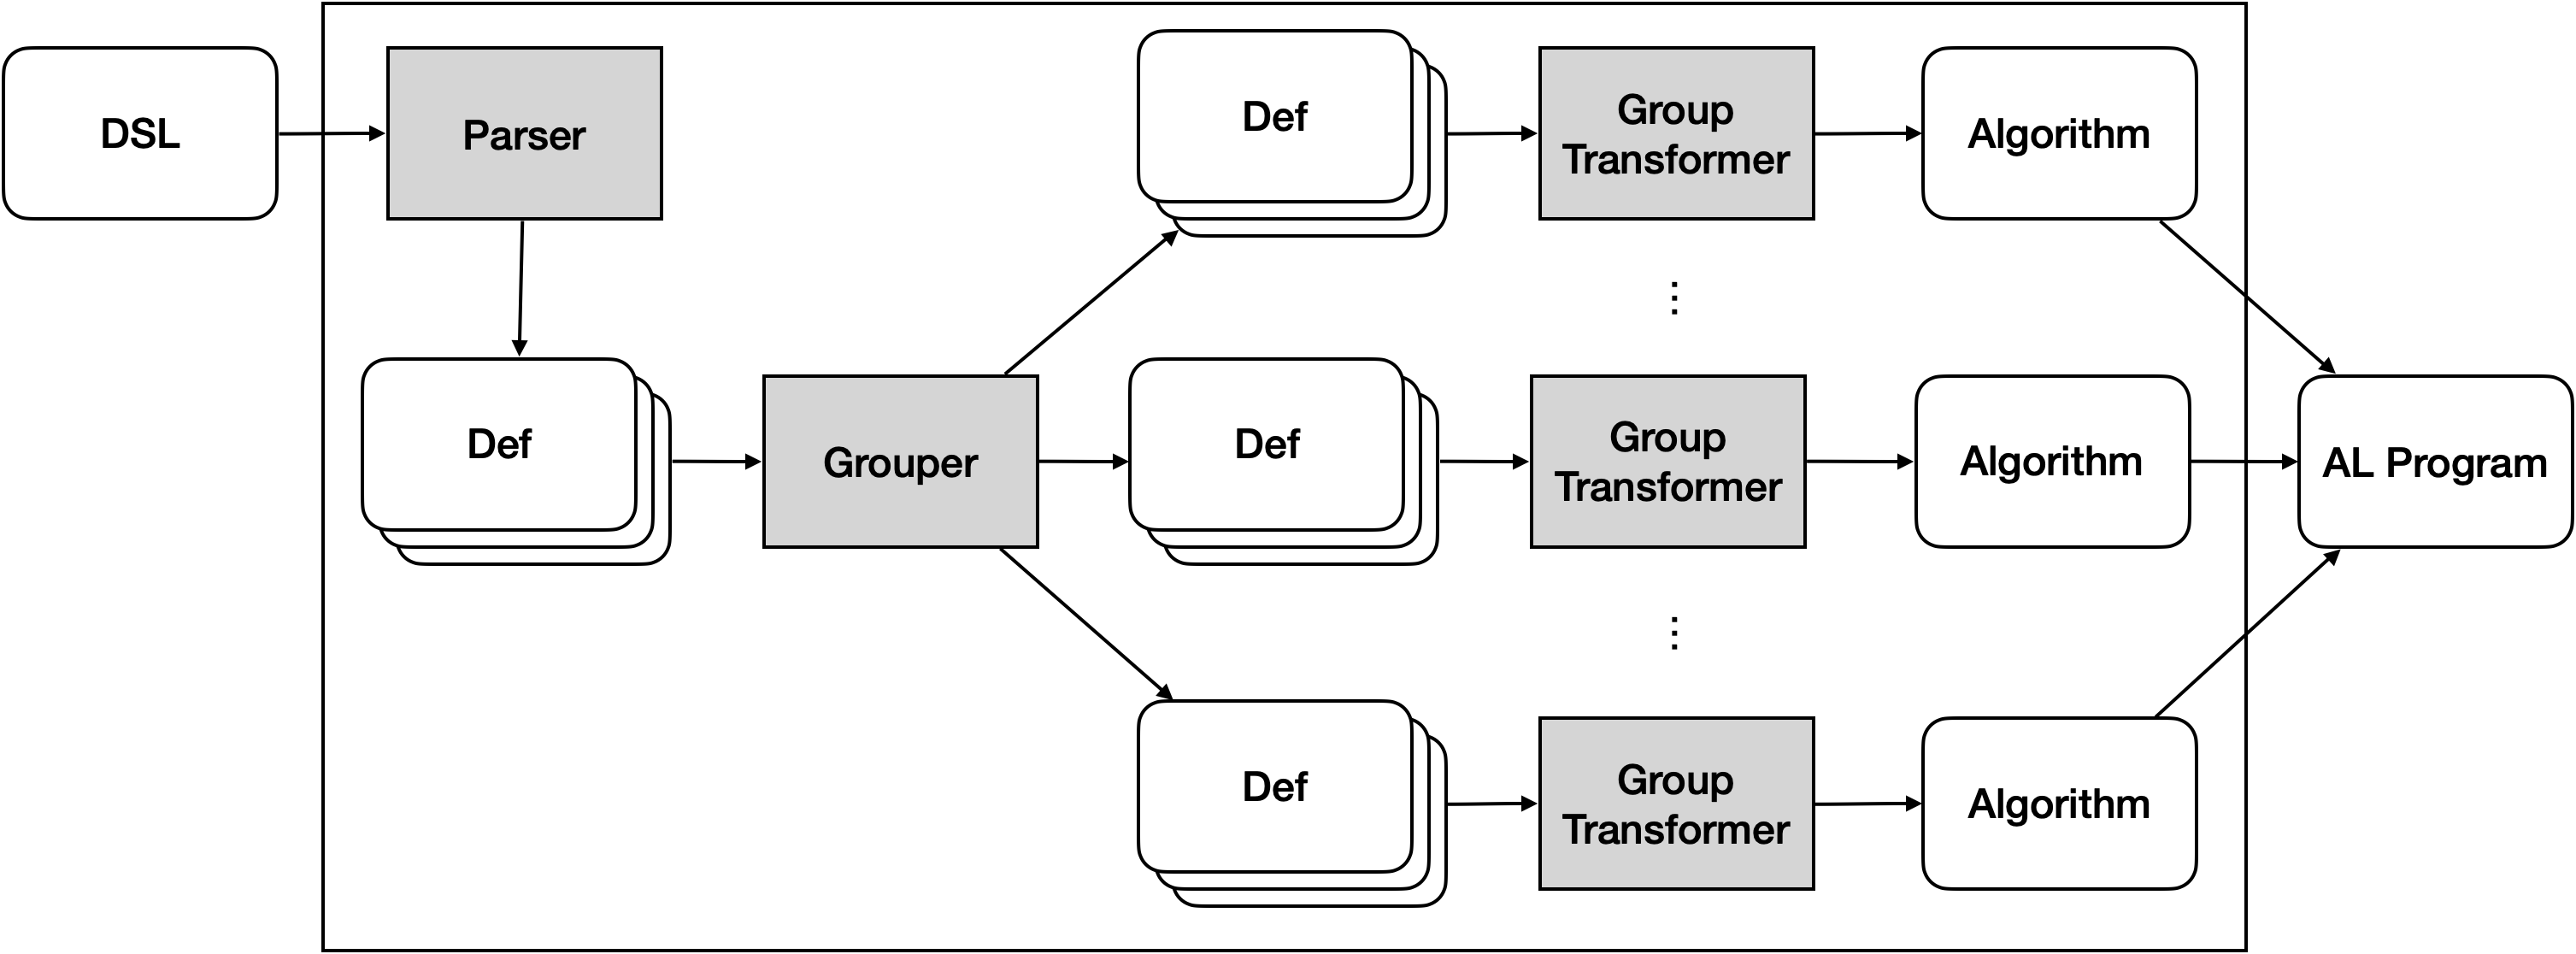
\includegraphics[width=\textwidth]{img/trans1}
    \caption{Overview}
    \label{fig:overview}
  \end{subfigure}
  \hfill
  \begin{subfigure}[b]{0.9\textwidth}
    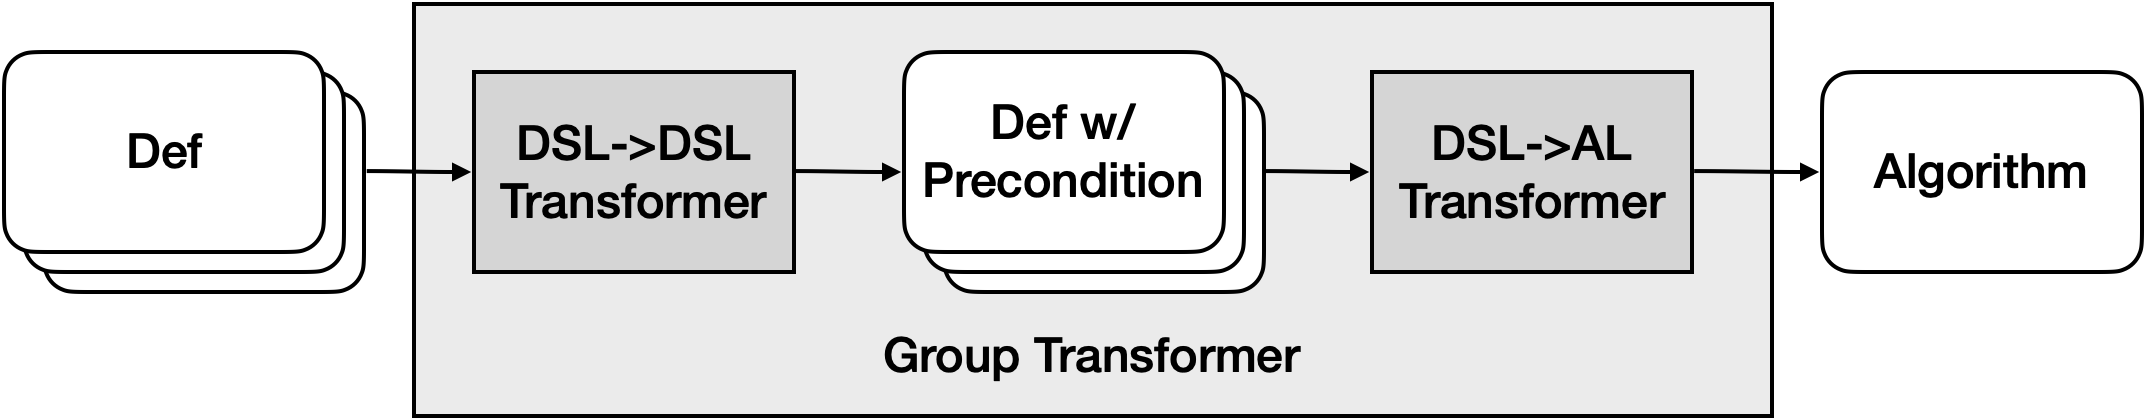
\includegraphics[width=\textwidth]{img/trans2}
    \caption{Group transformer}
    \label{fig:grouptrans}
  \end{subfigure}
  \caption{DSL->AL transformation}
  \label{fig:trans}
\end{figure}


Figure~\ref{fig:overview} shows the whole system of transforming DSL into an \al~program.
The input of the system is the \dsl~document,
and the output of the system is a single \al~program $\mathsf{p}$.
The input undergoes the following process of transformation.
First, the input DSL is parsed into a set of definitions: either a reduction rule or a
helper function. Then, the definitions are grouped. Reduction rules are grouped based on
their target Wasm instruction, and helper functions are grouped based on their names.
As a result, multiple groups are formed. Each group is transformed into a single algorithm,
$\mathsf{A}$. The transformed algorithms are collected into a single AL program, which is the
final output of this transformation system. This AL then can be stringified into a
prose notation to be rendered in the specification document, or can be coupled with the AL interpreter to form a Wasm interpreter.

Figure~\ref{fig:grouptrans} shows the detail of group transformer, a component of the Figure~\ref{fig:overview}.
The input is either a group of reduction rules \textit{r}, or a group of helper functions \textit{h}.
The output is a single algorithm.
Due to the fundamental difference between mathematical rules and algorithm,
directly transforming into an algorithm is a non-trivial task.
Therefore, the process is divided into two steps: first preprocess the DSL so that
it becomes more suitable for transformation, and then transform it into an algorithm.
As a first step, a group of definitions are first transformed into a different but equivalent group of definitions,
so that the new transfomred group of definitions satisfies certain \textit{preconditions}.
The preconditions are there to help generate AL algorithms with more ease.
If the input group already satisfies the precondition, then this transformation will keep the input intact.
Secondly, Then new group of definition is transformed into AL.
How the AL is generated slightly differ based on whether the group is a reduction rule group or a helper function
group, but they are both based on the following fundamental approach.
% Should I explain AL -> AL?

\subsubsection{DSL->DSL transformation}

There are two major steps for transforming DSL into DSL: 1. LHS/Parameter unification and
2. animation.

\textbf{1. LHS / Parameter Unification}

Unification is a step that makes all LHS (for reduction rule) or parameters
(for helper functions) identical within the group.
This precondtion already holds for most cases, with a few exceptions.
The most notable example is the `br` instruction.
Here are two simplified reduction rules for the `br` instruction
\[
r_1 = (..., [... \text{(BR 0)} ...]),  (..., ...), []
\]
\[
r_2 = (..., [... \text{(BR l+1)} ...]),  (..., ...), []
\]
The intention here is that `br l` instruction should be applied with different rule,
depending on whether l is 0 or not.
Note that the both rules do not have any premise. The condition check is implicitly assumed to be
done when mathcing the current configuration with LHS.

The following is the result of unification:
\[
r_1' = (..., [... \text{(BR t)} ...]),  (..., ...), [t = 0]
\]
\[
r_2' = (..., [... \text{(BR t)} ...]),  (..., ...), [t = l + 1]
\]
The temorary variable t is introduced for both rules, replacing 0 of the first rule and
l+1 of the second rule. In order to denote what the temporary variable originally was
in each rules, new premise is added, denoting t eqauls 0 in the first rule, and l+1 in the second rule.

\inred{
  TODO: Explain algorithm/methd of animation: walking two AST's simultaneoausly.
}


\textbf{2. Animation}

There are two problems that makes the transformation of premises into AL challenging.
First, if a given premise is an equality expression, then it may work as either a simple condition or
a binding of a new variable, and this should be inferred. More formally, it is required to
correctly find out where each free variable is getting bound. Second, the order
of premises can be permutated in an arbitrary order. This is problematic for
generating algorithm, since the exact order of steps are crucial in the algortihm.

Animation is a step that addresses these two challanges. Its goal is to infer
the bound variables and the order of each premise.
After animation, each premise is tagged with what variables it is binding
such that every variables are bound exactly once, and premises are ordered in a way that
all of unbound variables in each premise is already bound by the previous premises.

We have discovered that this solving the animation problem is in fact NP-hard.
We prove it by reduction from a known NP-hard problem, an exact cover problem.

Theorem: Animation problem is NP-hard.

Proof: \inred{TODO}

This theorem implies that there is no trivial method for solving this problem.
One obvious solution to this kind of problem is probably using a SMT solver such as Z3, since
this probelm is fundamentally a constraint problem.
However, using such a heavy tool seems to be a bit over-engineering for this rather small input.
Instead, we decided to use a simple yet effective approach.
We reduce the problem into a exact cover problem\footnote{Note that the direction is opposite with
the proof}, and then adopt the well-known effective algorithm to solve exact cover problem,
the Knuth algorithm[?].

\inred{
  TODO: Explain reduction to exact cover and Knuth algorithm to solve it
}.


\subsubsection{DSL->AL transformation}

In this section, we explain the transformation of DSL with preconditions into an AL algorithm.

----------------

Algorithm 1.

Input: A group of reduction rules r* = (lhs, rhs, prems)*

Output: An algorithm $\mathsf{A}$

1. lhs <- r*[0].lhs

2. instrs <- lhs\_to\_instr(lhs)

3. For r in r*:

--a. prems = r.prems

--b. rhs = r.rhs

--c. instr\_prems <- prems\_to\_instr(prems)

--d. instr\_rhs <- rhs\_to\_instr(rhs)

--e. instrs <- instrs ++ merge(instr\_prems, instr\_rhs)

4. (name, params) <- extract\_name\_and\_params(lhs)

5. Return ($\mathsf{algorithm}$ name (params) {instrs})

----------------

\inred{TODO: Pretty print algorithm 1}


After the group is tranformed, the next step is to
change each group into an algorithm. Algorithm 1 depicts the pseudocode of the transformation
of group of reduction rules into an algorithm.
First, the lhs of this reduction rule group is extracted on line 1, and is transformed into
an AL instructions on line 2. Since it is guaranteed that every lhs of reduction rule are
identical, any lhs from any rules of the group can be used. This transformed list of instructions
will be used as an initial list, and will grow iteratively by the loop on line 3.
Premises and rhs are extracted for each reduction rule on line a and b, and then transformed into
instructions on lines c and d. These two lists of instructions are merged to form a single
list of instructions, and then accumulatively appended to the intial instruction list.
Finally, the name and parameter of this algorithm should be extracted from the target instruction of the reduction rule,
which itself is obtained from any lhs of the rule on line 4. At last, the name, parameters, and
AL instructions will be packed and returned as the final algorithm.

\inred{
  TODO: Explain lhs\_to\_instr, prems\_to\_instr, rhs\_to\_instr, merge, extract\_name\_and\_params
}
